\chapter{Computational Tools in Quantum Information Theory}
\chaptermark{Computational Tools in QIT}

\par Traditionally physics research has been divided into "theoretical" and "experimental" physics: theoretical physics focusing on a rigorous mathematical framework for understanding our world and experimental physics concerned with testing the validity of the theories in a laboratory. With the increasing penetration of computers in how we do our work, the way we do physics research has inevitably experienced some changes. In recent years there has been a growing body of work in "computational physics" which is concerned with doing numerical experiments in a computer laboratory looking at how different theories should play out. This provides an intersection between theoretical and experimental physics where theories are analyzed numerically and the results are then compared to real world data from a laboratory. This has a great contribution in accelerating physics research. Some people call this approach "experimental mathematics". \cite{wolframexperimentalmath}
\par This chapter discusses some of the tools available to apply the techniques of computational physics to quantum information theory. As the situation is, physicists do not normally have the luxury of canned computer programs readily available for their work so they have to write the programs themselves. The "tools" talked about here are simply: programming languages and libraries/toolboxes to facilitate writing programs for a particular kind of problem.
\par Looking at the available programming languages we encounter many that we can potentially use to solve physics problems. There are C, C++, FORTRAN, Java, Python, MATLAB and Lisp just to name a few. Each of these has its own strengths and use cases where it excels. C and C++, for example, generate extremely fast compiled native code. Java programs, written once, can run on virtually any hardware. FORTRAN has a large body of legacy physics code. This project looks at two of these languages: MATLAB and Python.

\section{MATLAB}
MATLAB, which stands for MATrix LABoratory, is a self-contained proprietary programming environment developed by MathWorks to help scientists and engineers write numerical programming applications. As its name implies, it bases itself on matrices. It is a commercial product. By a self-contained environment we mean that it is a single package consisting of an integrated development environment tightly integrated with its own programming language and collection of libraries - or toolboxes as they are called. In this text when we refer to MATLAB, we will mostly mean the programming language.
\par MATLAB is a high level programming language designed for a special domain - i.e. scientific and engineering applications. In that it does a pretty good job. With its high level of abstractions it removes all the unnecessary worries of the underlying hardware. It has built in tools for plotting and simulations. It has a large collection of toolboxes pre-packaged for a variety of tasks ranging from solving differential equations to symbolic computing and digital signal processing. Additional toolboxes are also available which can be easily added and used. It also provides tools for designing basic graphical user interfaces for when the need arises.
\par Before we move on to the topic of quantum information toolboxes in MATLAB, we shall go through a basic tutorial of MATLAB to give the reader a feel of how it works. It is assumed that the user has a prior basic knowledge of working with any other programming language.

\subsection*{Tutorial: MATLAB Basics}
In this tutorial we shall be entering some basic commands at the MATLAB interactive prompt. \texttt{>>} is the MATLAB prompt and indicates that MATLAB is ready to accept an input command or statement. What shows up after entering the command is the output.
\par We start with variables. In MATLAB, variables are dynamically typed. That is, the type of the variable does not have to be declared before storing the value. Variables are also case sensitive.
\begin{verbatim}
>> a = 5
a = 
    5
>> b = 7
b = 
    7
>> B = 3
B = 
    3
>> a+b+B
ans = 
    15
\end{verbatim}
The basic data structure, of course, is a matrix. In fact the earlier examples are special cases of 1x1 matrices. Now let us use some vectors.
\begin{verbatim}
>> c = [1,5,3]
c =
   1   5   3

>> d = [4;3;7]
d =
   4
   3
   7

>> c*d
ans = 
      40

>> d*c
ans =
    4   20   12
    3   15    9
    7   35   21
\end{verbatim}
We can also select a particular element using indices.
\begin{verbatim}
>> d(1)
ans = 
      4
      
>> (d*c)(2,2)
ans = 
     15   
\end{verbatim}
We end our tutorial with a simple for loop.
\begin{verbatim}
>> for i=1:3
    disp(i)
   end

 1
 2
 3
\end{verbatim}
The more curious reader can consult one of the many detailed books on MATLAB. \cite{allendowneymatlab}

\subsection*{QI Toolboxes for MATLAB}
\par Due to MATLAB's popularity in academia over the years, a lot of research code has been written in MATLAB and a lot of people have written toolboxes for applications in science and engineering. This gives it a huge advantage as a programming language. For someone to understand and build upon such a previous work, learning MATLAB is a pre-requisite. A whole body of previous work is what keeps MATLAB relevant today.
\par Toolboxes have been written for quantum information work too. The following MATLAB toolboxes were explored as part of this project.

\subsection{QLib}
QLib is a free and open source toolbox written for quantum information research by Shai Machnes at the Tel-Aviv University \cite{qlib}. It provides a rich collection of functions to implement the ideas of QIT and explore questions with help from its visualization tools and optimization algorithms. Its features include simulating of quantum states including entangled states, various measures of entropy and entanglement, functions for measurements, Schmidt decomposition, gates, distance measures between density matrices, plotting and many more.
\par Let us take a look at some example code. This basic example parametrizes a random pure state and then performs the partial transpose entanglement test on it.
\begin{verbatim}
>> pure = param_pure_1_rand([2 2])
pure =
   0.4839 + 0.0000i
  -0.4078 + 0.0046i
   0.4005 - 0.3689i
  -0.5500 - 0.0236i

>> is_entangled_pt(pure)
ans =
     1
\end{verbatim}
\par This example plots the negativity vs concurrence of 10,000 random density matrices of two qubits.
\begin{verbatim}
neg = []; con = [];
for k=1:10000
    dm = param_dm_2x_rand([2 2]);
    neg(k) = negativity(dm);
    con(k) = concurrence(dm);
end
scatter(neg,con,2);
\end{verbatim}
The result is this plot.
\begin{figure}[H]
  %\begin{center}
    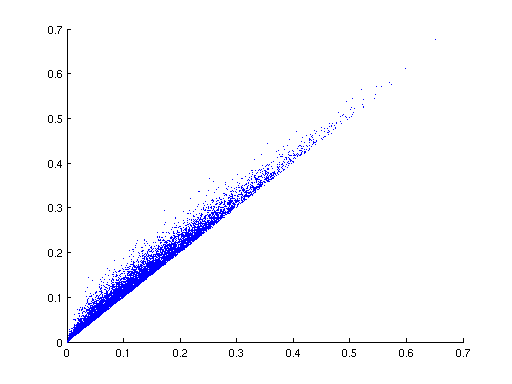
\includegraphics[scale=0.88]{figures/qlib-negativity-vs-concurrence.png}
    \caption{QLib: Negativity vs Concurrence of 10,000 random DMs.\newline X-axis: Negativity, Y-axis: Concurrence}
    \label{fig: QLib: Negativity vs Concurrence}
  %\end{center}
\end{figure}

\subsection{QETLAB}
QETLAB (Quantum Entanglement Theory LABoratory) is another free and open source toolbox for quantum information work. It was started and is primarily maintained by Nathaniel Johnston at the Mount Allison University, Canada \cite{qetlab}. As its name implies, it specifically aims to provide functionality related to entanglement. The goal of the project is to remain up to date with an ever-growing catalogue of separability criteria, positive maps, and related functions of interest. Compared to QLib, this toolbox is more recent and is under active maintenance at the time of this writing.
\par Let us look at some example code. This example generates a random 2x2 density matrix and calculates its von Neumann entropy.
\begin{verbatim}
>> rho = RandomDensityMatrix(2)
rho =
   0.83755 + 0.00000i  -0.01727 - 0.00114i
  -0.01727 + 0.00114i   0.16245 + 0.00000i

>> Entropy(rho)
ans =  0.63909
\end{verbatim}

This example generates a random state vector and then calculates its Schmidt decomposition.
\begin{verbatim}
>> d = 2
d =  2
>> phi = RandomStateVector(d^2)
phi =
   0.35227 + 0.32456i
  -0.37642 + 0.23467i
  -0.22955 - 0.66080i
   0.17927 - 0.22872i

>> [s,u,v] = SchmidtDecomposition(phi)
s =
   0.96858
   0.24872

u =
  -0.64481 + 0.00000i   0.76434 - 0.00000i
   0.73711 + 0.20221i   0.62184 + 0.17058i

v =
  -0.547168 - 0.671034i   0.055448 - 0.497238i
   0.339278 - 0.367710i  -0.865439 + 0.026381i

\end{verbatim}
The entries of \texttt{s} are the Schmidt coefficients and the columns of \texttt{u} and \texttt{v} are the left and right Schmidt vectors respectively.

\subsection{Quantum Information Toolkit}
Quantum Information Toolkit is an open source quantum information toolbox available for both MATLAB and Python developed by Ville Bergholm et al. \cite{quantuminformationtoolkit}. Its MATLAB and Python versions both contain equivalent functionality. We shall discuss it in detail in the Python section.

\pagebreak

\section{Python}
Python \cite{python} \cite{primerscientificpython} is a free and open source, multi-paradigm, general purpose programming language. By multi-paradigm we mean that it can be used to code in the procedural, object oriented or functional programming styles. It is cross-platform and can run from desktops and servers to mobile devices and even small embedded systems like network routers or miniature computers like the Raspberry Pi. This gives it the flexibility to be used in pretty much any environment for almost any purpose. We find it being used in desktop and server applications, industrial automation, robotics, scientific research and control systems. In scientific research it can be used for mathematical modeling, simulation, laboratory automation, signal processing, data analysis and numerous other tasks.
\par Python's design philosophy makes it very easy to learn the language and also makes it easy to read and understand other people's code. Furthermore, its high level abstractions make it an ideal language for rapid prototyping. This makes it an attractive language to implement scientific ideas in. Hence over the years, it has accumulated a vast collection of libraries to do many kinds of scientific computations. In addition to that, it also has a large collection of libraries to help with many other kinds of programming. Hence the researchers who learn Python also have access to a lifetime supply of tools to implement their ideas in any way they like: be it providing a web interface to their signal processing tool, writing a good looking graphical interface to present their research, plotting their data in a variety of forms or explaining their code step by step in an iPython notebook. They have numerous options to make their research more immediately useful to the community. This makes Python an increasingly popular programming language within the scientific community.
\par Before we proceed to discuss the quantum information toolboxes available for Python, we should briefly mention the popular libraries NumPy, SciPy and SymPy which have become ubiquitous among the scientific programming community. Many of the other scientific libraries build on top of these.

\subsection{NumPy}
Numpy \cite{numpy} adds support for large multi-dimensional arrays and matrices to Python. It also provides a large library of mathematical functions to operate on those arrays. It is the go-to library for Python when dealing with large scale number-crunching and contains very powerful mathematical functions. NumPy is free and open source software and many other numerical solutions for Python build on top of NumPy.
\par Let us look at a simple example of solving some basic linear algebra problems.
\begin{verbatim}
>>> import numpy as np
>>> from numpy.linalg import solve, inv
>>> a = np.matrix([[2.4,3.5,1.3],[6.2,7.1,3.9],[5.5,9.0,8.4]])
>>> a.transpose()
matrix([[ 2.4,  6.2,  5.5],
        [ 3.5,  7.1,  9. ],
        [ 1.3,  3.9,  8.4]])
>>> inv(a)
matrix([[-0.92485113,  0.66706867, -0.16657873],
        [ 1.15436798, -0.49031431,  0.04899374],
        [-0.63126555,  0.08856561,  0.17562373]])
>>> b =  np.array([3, 4, 5])
>>> solve(a, b)    # solve for equation ax = b
array([-0.93917238,  1.74681541, -0.66141554])
\end{verbatim}

\subsection{SciPy}
SciPy \cite{scipy} is a more general scientific programming library for Python. It builds on top of NumPy and adds its own huge library of modules and functions for many tasks common in science and engineering. Some of these tasks are optimization, linear algebra, integration, interpolation, special functions, fast Fourier transform, signal and image processing and ordinary differential equation solvers. Like NumPy, SciPy is also free and open source software.

\subsection{SymPy}
SymPy \cite{sympy} is a Python module for symbolic computations, unlike NumPy discussed earlier which is built for numerical computations. By symbolic computations, we mean computations of mathematical objects symbolically: the mathematical objects are represented exactly, not approximately, and mathematical expressions with unevaluated variables are left in symbolic form.
\par Let us look at an example of a basic integral.
\begin{verbatim}
>>> from sympy import *
>>> x = symbols('x')
>>> integrate(exp(x)*sin(x) + exp(x)*cos(x), x)
exp(x)*sin(x)
\end{verbatim}
We see that rather than requiring or computing the numerical value for $x$, it is treated in symbolic form.
\par Just like NumPy and SciPy, SymPy is also free and open source.

\subsection{matplotlib}
matplotlib \cite{matplotlib} is an open source plotting library for Python. It is normally used with NumPy to produce high quality plots of mathematical functions and scientific data. SciPy also makes use of it. matplotlib's pyplot interface provides an interface very similar to MATLAB's plotting.
\par Let us look at a basic plotting example.
\begin{verbatim}
>>> import numpy as np
>>> import matplotlib.pyplot as plt
>>> x = np.linspace(0, 1, 100)
>>> y = np.sin(4 * np.pi * x) * np.exp(-5 * x)
>>> plt.plot(x, y)
>>> plt.grid(True)
>>> plt.show()
\end{verbatim}
This results in the following plot.
\begin{figure}[H]
  \begin{center}
    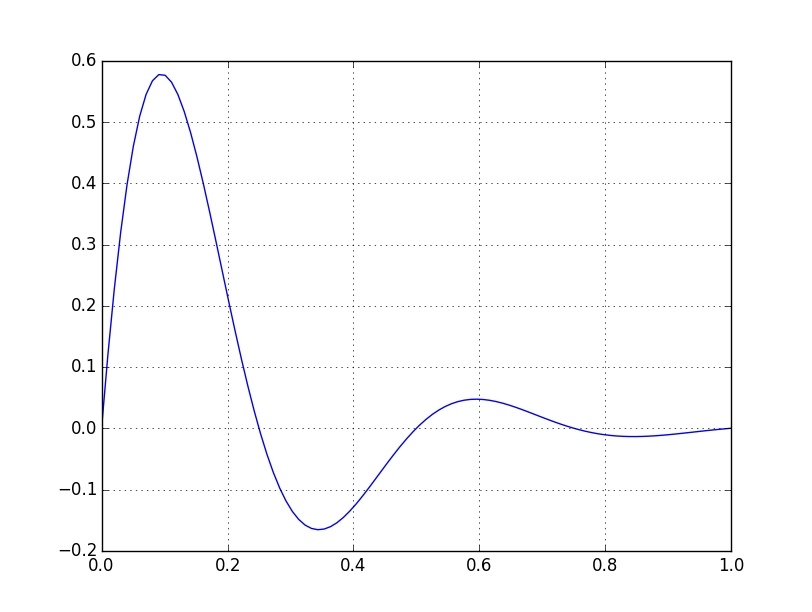
\includegraphics[scale=0.55]{figures/matplotlibexample.png}
    \caption{Plotting with matplotlib}
    \label{fig: matplotlib Example}
  \end{center}
\end{figure}

\par Now that we have become familiar with the more essential and more popular scientific modules in the Python ecosystem, we shall proceed to discuss the ones specific to quantum information theory.

\subsection{qitensor}
qitensor is a quantum information module for Python written by Dan Stahlke \cite{qitensor}. It is based on NumPy and adds functionality to facilitate working with finite dimensional quantum mechanics of many particles. It also has preliminary support for symbolic calculations through SymPy.
\par A simple example using qitensor:
\begin{verbatim}
>>> from qitensor import qubit
>>> ha = qubit('a')
>>> hb = qubit('b')
>>> ha * hb
|a,b>
>>> x = (ha * hb).array()
>>> x
HilbertArray(|a,b>,
array([[ 0.+0.j,  0.+0.j],
       [ 0.+0.j,  0.+0.j]]))
\end{verbatim}

\subsection{Quantum Information Toolkit}
Quantum Information Toolkit, developed by Ville Bergholm et al. \cite{quantuminformationtoolkit}, is a free and open source quantum information toolbox for both MATLAB and Python. The MATLAB and Python versions both contain equivalent functionality. The Python version builds upon the NumPy, SciPy and matplotlib libraries.
\par Some example code from the Python version:
\begin{verbatim}
>>> a = state('0')
>>> b = state('1')
>>> a.measure()
(array([ 1.,  0.]), 0)
>>> b.measure()
(array([ 0.,  1.]), 1)
>>> a * b.transpose() 
array([[ 0.,  1.],
       [ 0.,  0.]])
dim: (2,) <- (2,)
>>> ab = tensor(a,b)
>>> ab.data
array([[ 0.],
       [ 1.],
       [ 0.],
       [ 0.]])
\end{verbatim}

\subsection{Quantum Toolbox in Python (QuTiP)}
QuTiP \cite{qutipdoc} is a very large free and open source toolbox for simulating open quantum systems. Started by Robert J. Johansson of RIKEN Japan and Paul D. Nation of Korea University, it has grown into a large collaborative project involving researchers from many other institutes. Like many toolboxes previously discussed, it also builds on top of NumPy and SciPy and uses matplotlib for plotting. It also optimizes for speed by using Cython to make Python code many times faster and by parallelizing tasks when possible.
\par Unlike the other toolboxes discussed so far, this one is not specific to quantum information. However it does have a great internal structure and a huge library of functions to simulate a wide variety of quantum systems. The efficiency in terms of computation time is also very good. On top of that, it is actively maintained, widely used and has a larger community to get help from. This makes it a good choice as a toolbox to implement quantum information functions in.
\par Extending QuTiP with quantum information functionality is the main theme of this project. Hence the whole next chapter is dedicated to it. The next chapter starts with the basics of how QuTiP works and how more functions can be written on top of it. Then it demonstrates the code written for this project, including the addition of QI functions to QuTiP and making use of them in simulations.
\par For now, we can use a simple example as an introduction, dealing with these two states.
\begin{align*}
\ket{\psi_0} &= \ket{\uparrow} \\
\ket{\psi_1} &= \frac{1}{\sqrt{2}} \left( \ket{\uparrow} + \ket{\downarrow} \right)
\end{align*}

\begin{verbatim}
>>> from qutip import *
>>> import numpy as np
>>> up = basis(2,0)
>>> dn = basis(2,1)
>>> psi0 = up
>>> psi1 = 1/np.sqrt(2) * ( up + dn )
>>> print(psi0)
Quantum object: dims = [[2], [1]], shape = [2, 1], type = ket
Qobj data =
[[ 1.]
 [ 0.]]
>>> print(psi1)
Quantum object: dims = [[2], [1]], shape = [2, 1], type = ket
Qobj data =
[[ 0.70710678]
 [ 0.70710678]]
>>> # The density matrix for an equal mixture of both states
>>> rho = 0.5 * ( ket2dm(psi0) + ket2dm(psi1) )
>>> print(rho)
Quantum object: dims = [[2], [2]], shape = [2, 2], type = oper, isherm = True
Qobj data =
[[ 0.75  0.25]
 [ 0.25  0.25]]
\end{verbatim}

